\documentclass[11pt]{article}
\usepackage{a4, fullpage}
\usepackage{bibtopic}
%\usepackage[small,compact]{titlesec}
\usepackage{float}
\usepackage{amssymb,amsmath}
\usepackage[T1]{fontenc}
\usepackage{graphicx}
\usepackage{multicol}

\restylefloat{table}
%\usepackage{parskip}
%\usepackage{setspace}

%\setlength{\parskip}{0.3cm}
%\setlength{\parindent}{0cm}
%\setlength{\textheight}{10in}
%\setlength{\textwidth}{6.5in}
%\setlength{\parskip}{2pt}
%\addtolength{\oddsidemargin}{-.3in}
%\addtolength{\evensidemargin}{-.3in}
%\addtolength{\topmargin}{-.6in}
%\addtolength{\textwidth}{.6in}

%Crowdsourcing of tasks has become very popular. It is often based on the principle that by having many different contributors to performing a task, an accurate and appropriate result will be achieved. The classical example is wikipedia where popular pages tend to be more accurate than less popular one. But contributions to a task do not always come for free and frameworks such as Amazon's mechanical turk allow for monetary rewards to be paid in exchange for contributing or performing a task. It is therefore the case that fewer contributions from more trustworthy contributors is more effective than many contributions from less trustworthy sources. 

%The aim of the project is to design and implement a framework that allows the optimum number of contributors to be selected on the basis of their trustworthiness for a desired accuracy of the outcome/result and that evaluates the trustworthiness of contributors on the basis of the accuracy of the results they provide.


\begin{document}



\title{Crowdtrust - Trustworthy Information From The Crowd\\ Group Project }

\author{Giovanni Charles \and Adam Fiksen \and Ryan Jackson \and Sahil Jain \and John Walker \and \\ Emil Lupu}

\date{\today}         % inserts today's date

\maketitle           % generates the title from the data above
\newpage


\begin{abstract}
\noindent Outsourcing is becoming increasingly popular in a lot of areas and, as a result, providing these required services has 
become big business. Companies are using the Internet to accept jobs from requestors which often require some human intelligence ,
such as tagging images. They then distribute these jobs to a crowd of workers and return the results to the requestor. This process is called
crowdsourcing. %Not happy with this
\\
\\
\noindent At the moment Amazons \emph{Mechanical Turk} is the only real crowdsourcing `giant' in the market. With over 500,000 workers it offers
anyone with a computer and internet connection the ability to `earn \$\$\$ while working from home!'. Requestors (companies or individuals) 
can submit a HIT (Human Intelligence Task) to the Mechanical Turk system. This HIT is then displayed to all users along with a 
reward for its completion. Upon completion, the results are then sent back to the requestor and they decide whether the work is worth paying for. 
This system raises a problem for requestors though, `how do I know how accurate my results are?'. You have no control over which worker selects your HIT and
your task of `Transcribe this podcast' could be carried out by someone unqualified for the job (e.g. they don't speak English). The solution
most requestor guides offer is to submit your job to numerous workers, but this pushes up your costs linearly and leaves a difficult
decision on the number of workers to consult.
\\
\\
We seek to create a solution to this problem by providing a framework in which requestors can submit jobs with a required level of accuracy. Our
system dynamically decides how many users it needs to consult to achieve this based on their expertise. 
  
\end{abstract}

\newpage

\tableofcontents	%Do contents page and a 1 page break afterward

\newpage

%%%%%%%%%%%%%%%%%%%%%%%%%%%%%%%%%%%%%%%%%%%%%%%%%%%%%%%%%%%%%%%%%%%%%%%%%%%%%%%%

\section{Executive Summary}

\subsection{What is our product?}
Let's say that I have a 100 photos of birds, and I want to know which birds are 
robins, but I have no prior knowledge of birds. Our product, CrowdTrust, focusses
on providing a solution for this problem.

Our product provides a framework for a user to submit a task and specify
the level of accuracy they want achieved in the task. At the moment,
there is only one main competitor in the market, Amazon's Mechanical
Turk. Our product aims to improve on Mechanical Turk by prioritising responses
from experts as well as dynamically deciding when a task is completed (based
on the responses and desired accuracy).

So how does our product tie in with the problem previously posed? CrowdTrust
provides us with the environment to upload the photos of birds and ask the question
"Which of these are 
robins?", specify the level of accuracy desired (say, with 95\% certainty), and then 
the task is sent out to the crowd. Once completed, a solution to the 
task as proposed by the crowd is returned, indicating which birds are robins.

\subsection{Why now?}
Crowdsourcing is become more popular day by day. It allows a person who needs
a job done, but has no prior knowledge on the subject, to get a very accurate
result through the contribution of many people who might be experts on the
subject of the task. Besides Mechanical Turk, there are other websites which
provide a specialised crowdsourcing frameworks, such at Stack Overflow. We wanted
to produce a framework which would not necessarily be specialised. The scope of
problems people face with today is large, and we wanted to take advantage of this.
%Write what crowdrust currently does .. image processing etc

\subsection{Why would you want it?}
There are two types of users who can use CrowdTrust. Firstly, there is the client,
who is the person who submits a task which needs answering. A client would want
to join because they could receive an accurate solution to a problem which they
wanted solving. Also, in the future, when paying the crowd is implemented,
using CrowdTrust could be significantly cheaper than Mechanical Turk. The second
type of user are the crowd members. Crowd members would want to join because
they might have a passion for solving problems. With the scope of CrowdTrust,
the types of problems you solve is massively varied. As mentioned, eventually, the crowd
would also be paid for solving tasks, which would be a primary reason as to why
someone would solve problems.
%%%%%%%%%%%%%%%%%%%%%%%%%%%%%%%%%%%%%%%%%%%%%%%%%%%%%%%%%%%%%%%%%%%%%%%%%%%%%%%%
\newpage
\section{Introduction}
%Set the scene ( motivation )
%State the problem you are trying to solve ( Ojective(s) )
%Summarise what you achieved ( contributions )
%%%%%%%%%%%
\subsection{What Is Crowdsourcing} %Change the I adam and 'I' will kill you
Our project concerns \emph{crowdsourcing}. `the book' would describe crowdsourcing as the principle of obtaining an accurate 
and appropriate result by having many different contributors performing a task, but we'd like to start with a story which
we believe encapsulates the idea of crowdsourcing in its most positive and useful light.

In January 2009 Timothy Gowers (Fields Medal winner and avid blogger) used his blog to post a striking question \emph{Is massively 
collaborative mathematics possible?}. He posted a difficult and unsolved mathematical problem he was particularly interested in and invited 
people to contribute to its solution in the comments section. The project initally got off to a slow start but once the ice was broken the 
comments flooded in. 37 days , 27 contibuters and 800 comments later Timothy Gowers was able to announce that not only had they solved the 
original problem but they had also solved a harder generalisation of it, he called his experiment the \emph{Polymath Project}.[6]

This is a nice example of how crowd sourcing can be used to combine the skills of many individuals and produce answers to complex problems,
but there are many motivations to outsource your task to the crowd:
\begin{itemize}
\item
\emph{Computational Difficulty:} Timothy Gowers provided a nice example of a computationally difficult problem. It is extememly unlikely you
would be able to write a program or use Wolphram Alpha to produce a complex mathematical proof, some problems require what we like to call
the `human touch'. Problems which require the human touch are in no way confined to the realms of complex mathematics. Identifing an unknown
bird in a picture, for example, would prove quite difficult. On a computer, it may be possible to utilise a program such as Google Goggles, but even then you 
would probably need a good quality photograph, whereas one avid bird enthusiast in the crowd might be able to easily identify the bird and
return the correct answer.
\item
\emph{Saving Time:} In 2009 aviator Steve Fosset crash landed deep in the Nevada desert, his friends knew they had a very small
and time critical window to find him alive and they had little faith in the current search and resuce operations. They organised for satellite 
images to be taken of the desert and the images were passed to a crowd who were asked to identify foreign object which could be potential crash 
sites.[7] This is a nice example of how the crowd can be used to literally cover a large amount of ground in a small amount of time. Not all 
examples of saving time are quite this dramatic though. Image tagging is an extemely arduous task for an individual or small group of people 
to perform, and tagging a relatively large set of images could take weeks or even months; outsourcing this to the crowd could have the job 
done in a number of hours.
\item
\emph{Saving Money:} `Time is money' as they say and this goes hand in hand with the point above. If you have to pay a team of high salary computing
professionals to tag images for your project when you could be paying them to write code this is not cost effective, however passing this job off
to a crowd of lower paid people could potentially save you a lot of money. 
\item
\emph{Reaching A Willing Audiance:} Unless it's something they enjoy, people unfortunately are not willing to work for free. This is why
getting the general public to do things such as complete surverys can be difficult. The
crowd members will be incentivised to perform work and as such will be more likely to complete a task.
\end{itemize}

%%%%%%%%%%%
\subsection{General Problem Description}
\begin{enumerate}
\item
\emph{How do we get these problems to the crowd?} 
\\
It is unlikely many people with a problem to be solved would want to go to the trouble
of creating a crowd themselves, as this would be comparable to the complexity of the problem itself, therefore there is a need for a third party
crowd management system. 
\item
\emph{What problems can we ask the crowd?} 
\\
Specialised crowds have been successful and certainly have their uses. For instance 
\emph{www.stackoverflow.com} can be thought of as a crowd specialising in the solution of computing problems. It is unlikely, however, that a community exists which specialises in indentifying bird pictures or to search satellite images for crash sites, therefore access to a generalised crowd, able to adapt to, and solve, a wide variety of problems, is desired. The crowd management party therefore needs to provide
the ability to ask a wide variety of questions and the ability to easily encorporate new questions in response to new technology.
\item
\emph{How many people do we ask, who do we ask and how can we trust what they say?} 
\\
Crowd members will be a representative sample of the general 
population, some will be brighter than others and some will be willing to put in more effort than others. Based on this all 
annotators can be placed on a scale of trustworthiness, rating how much an answer they give can be believed. This raises the question of `how many 
people do I ask?'; is consulting a small number of very trustworthy people better than a large number of average trustworthy people? However, the same subset of experts
can't be asked over and over again as workload will build up and answers will be delayed. If there is a 
`specialist' question, is it directed to someone with knowledge of that specialism? Clearly a sophisticated algorithm is needed on the crowd
management side to address these problems. 
\end{enumerate}


%%%%%%%%%%%
\subsection{Analysis of the Current Marketplace}
At the moment, there are a few crowdsourcing platforms in the market. These
are discussed below.

\subsubsection{Amazon's Mechanical Turk}
Amazon's Mechanical Turk, or MTurk as it is commonly known is by far the most well known
internet crowdsourcing platform. MTurk allows `requestors' to submit jobs to the 
system which are then solved by a group of around 500,000 `turkers'[8]. For each 
complete job, they are rewarded with a payment which is usually around 20 cents.
Mechanical turk offers no real garuntee of accuracy 
with its service and many people choose to submit their jobs multiple times to the
system themselves to validate them -- this obviously entails multiple payments.[9]


\begin{figure}[htbp]
\begin{center}
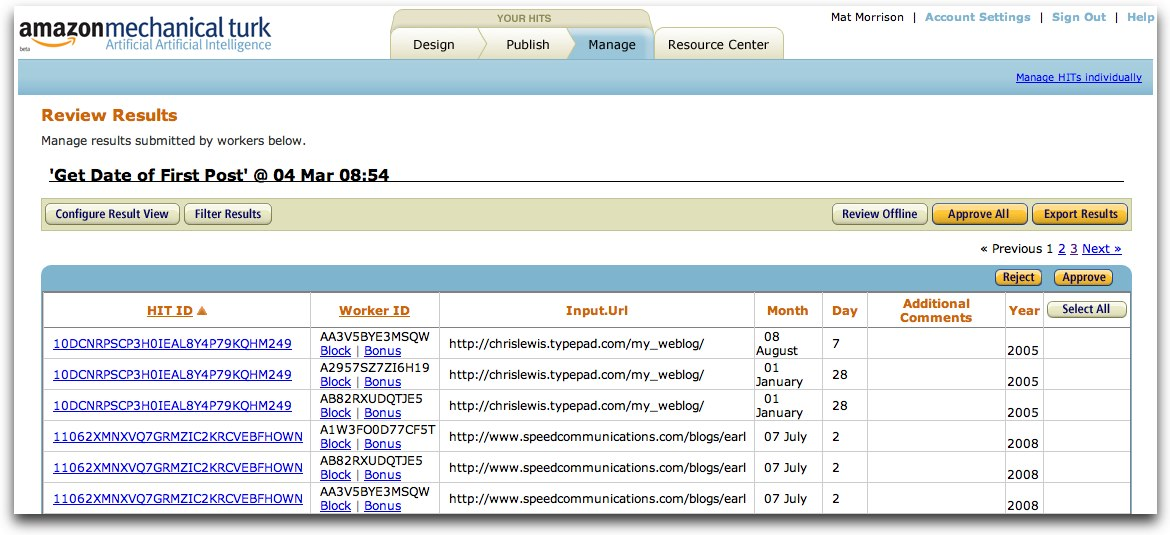
\includegraphics[width=\linewidth]{images/mturkinterface.jpg}
\caption{MechanicalTurk Interface}
\label{default}
\end{center}
\end{figure}



\subsubsection{Microworkers}
Microworkers is very much similar to MTurk, however Microworkers gives submitters the 
option to rate the crowd members work and the crowd members must maintain their rating above 75\% at
all times. [10]

There are also many others such as CrowdFlower and Elance that follow in a similar vein to MTurk.

\begin{figure}[H]
\begin{center}
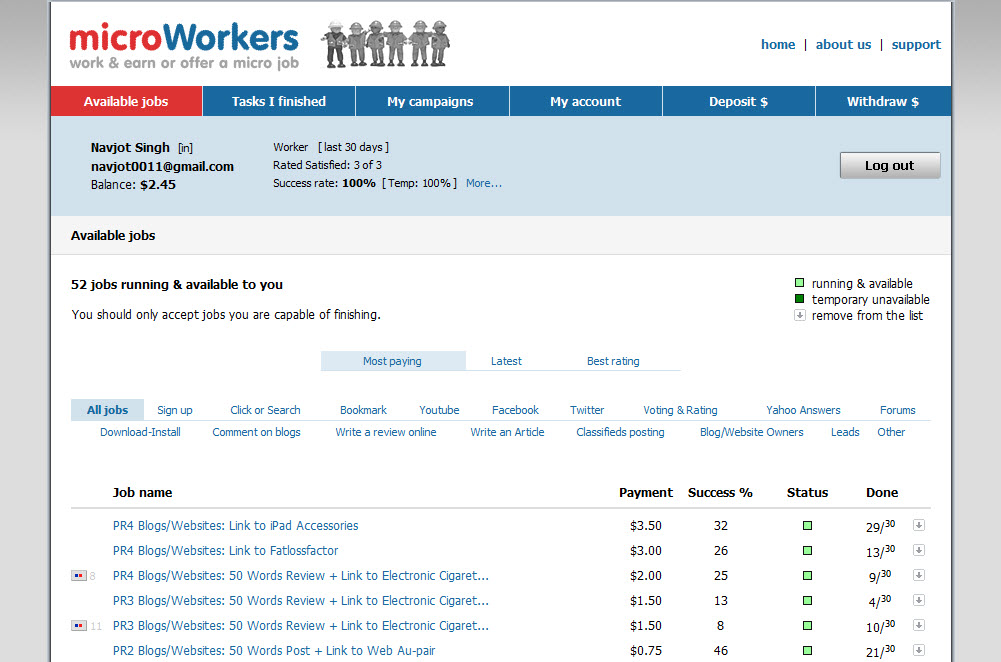
\includegraphics[width=\linewidth]{images/microworkersinterface.jpg}
\caption{Microworkers Interface}
\label{default}
\end{center}
\end{figure}


\subsection{Crowdtrust}
Although MTurk offers a very complete platform, with the ability to upload and answer a wide variety of questions,
it takes a very naive approach to making sure the requestor gets what they actually want. MTurk simply offers the requestor
the choice of not paying if they're dissatisfied with the work. The requestor has to do any validation of the answers themselves. 
Microworkers goes some way to addressing this problem by giving the crowd a success rating, however all this achieves is banning a crowd
member if they blindly answer questions -- it gives the requestor no confidence in their answer.
\\
\\
Crowdtrust seeks to provide a solution to this we aim to:

\emph{Design and implement a framework that allows the optimum number of contributors to be selected on the basis of their trustworthiness 
for a desired accuracy of the outcome/result and that evaluates the trustworthiness of contributors on the basis of the accuracy of the 
results they provide.}

\begin{figure}[H]
\begin{center}
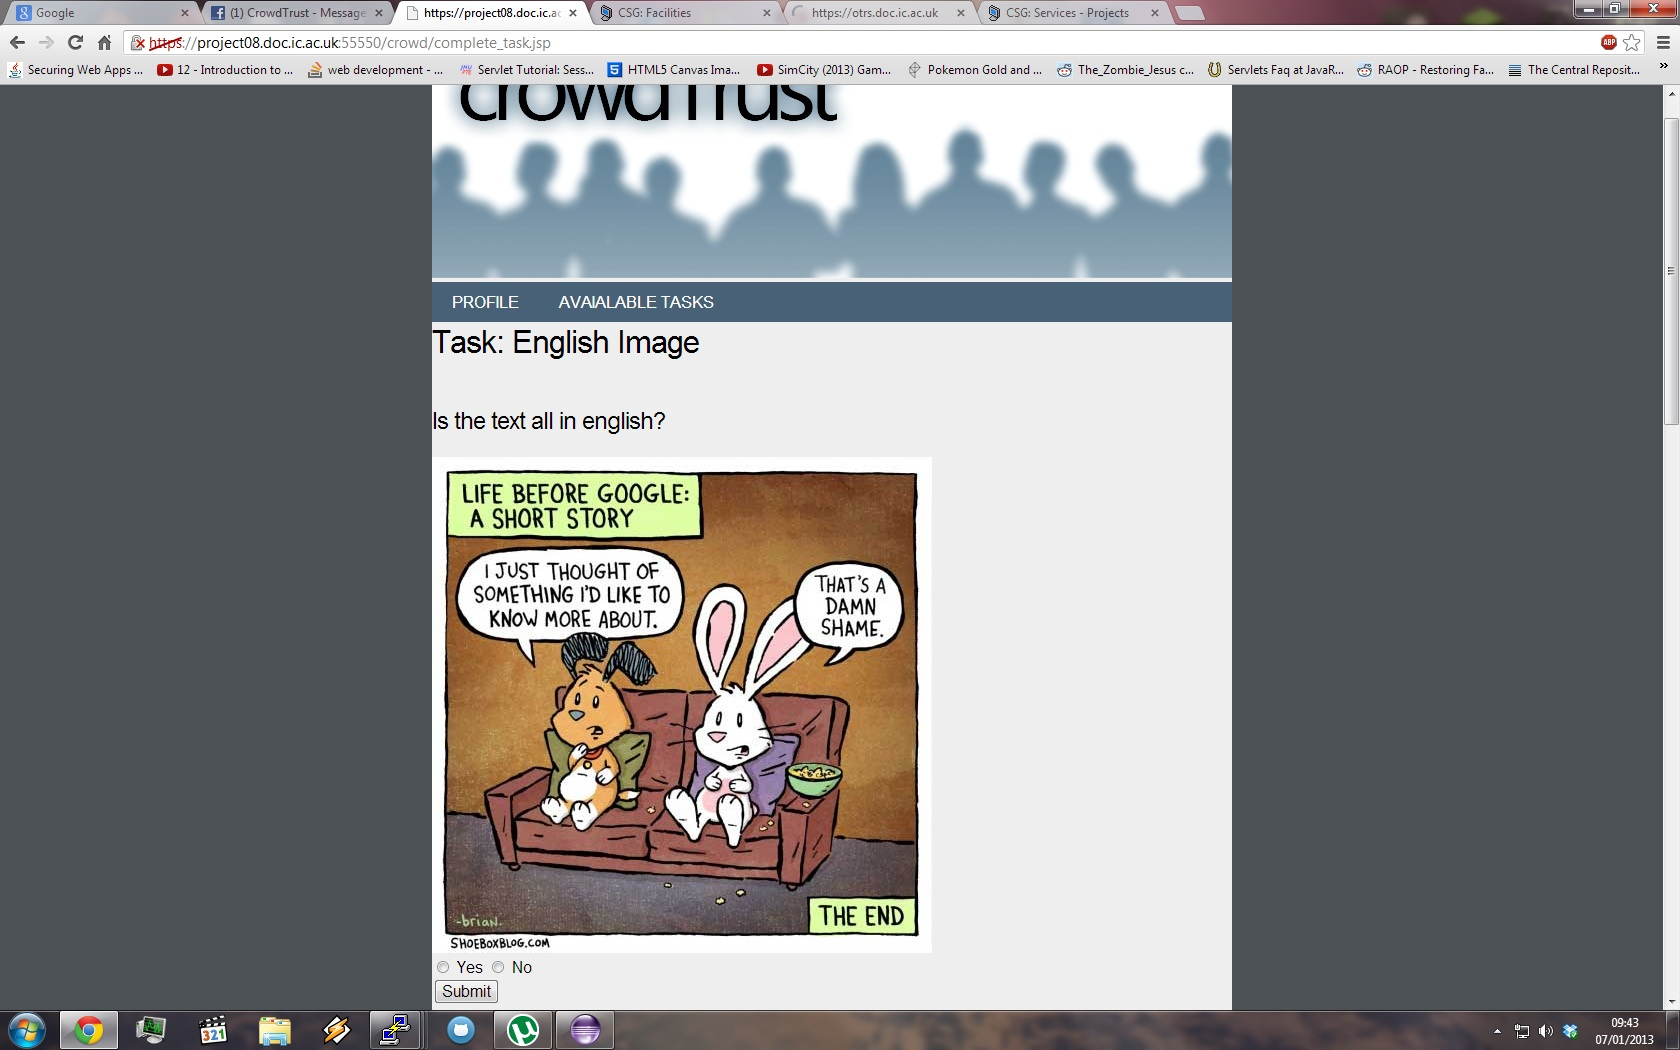
\includegraphics[width=\linewidth]{images/crowdtrustinterface.jpg}
\caption{Crowdtrust Interface}
\label{default}
\end{center}
\end{figure}

%%%%%%%%%%%
\subsection{Formal Objectives}
We seek to complete the following objectives
\begin{enumerate}
\item
%Generalise media
\item
%Generalised input
\item

\item

\item

\end{enumerate}



%%%%%%%%%%%%%%%%%%%%%%%%%%%%%%%%%%%%%%%%%%%%%%%%%%%%%%%%%%%%%%%%%%%%%%%%%%%%%%%%
%\newpage
\section{Design and Implementation}
% Detail your design why did you do it this way?
%Summarise Key implementation details (how did you do it what 
%tools did you use
%%%%%%%%%%%
%%%%%%%%%%%
\subsection{Framework}
% ADAM FIKSEN / RYAN 
\subsubsection{Client Design and Implementation}
On the side of the client, the web pages are generated from html5/css and jsp. 
Our site contains a persistent theme throughout, with the crowdtrust header and
created by footer appearing on every page, and other modules appearing depending
on location (e.g. the nav bar changes once a user is logged in). This was achieved
utilising \emph{sitemesh} [http://wiki.sitemesh.org/display/sitemesh/Home]
which provides a framework enabling the use of the Gang of Four decorator pattern.
As a user moves between contexts, the pages they can navigate to are modified
to fit with their intention -- from the homepage, pages of information about
crowdtrust can be accessed easily, whereas once logged in as a client, the user
is presented with links to adding tasks etc. Logging out will return them to
the homepage with general information again.

As a client user, tasks are submitted with information such as `task question'
and `media type' (submitting an incorrect media type will invalidate the task).
Once added, tasks are retrieved in the `upload subtasks' page via a servlet call,
allowing the user to submit subtasks to any previously created task. To save time,
the user may also upload a zip file contatining any number of files to add to the task.
The client can then observe various statistics about their tasks from their tasklist page,
also retrieved through a servlet call.

As a crowd user, a list of available tasks is displayed. The
contents of this list depend upon the user skill level, tasks they've completed
etc., with the call for retrieving the correct tasks being sent server side. From
this list a user selects a single task to do, which takes them to a page displaying
a random subtask of the task. This subtask is displayed through inline jsp, which
checks the media type of the task and uses the appropriate html tag (<img> for images etc.).
The possible answers are diplayed similarly. Upon submitting an answer, the response
is sent to the server and a new subtask is retrieved until no more remain, resulting
in a redirect to the tasklist.

\subsubsection{Server Implementation}
Almost every page has some interaction with our servlet through the use of jsp.
Many pages will query the database to retrieve subtasks or user information and for
this we have used inline jsp -- we have conformed to the MVC design pattern, keeping
our business logic separate from our view. For more in depth tasks, such as
adding users, tasks and subtasks, and also responding
to these tasks, we have implemented the functionality in Java. Whenever these servlets
are called, the user's session is validated initially (redirecting to index if not),
followed by calls to the database as required. The database calls have all been placed
in the package `db' to separate interaction with the db from interaction with the webpages.
On the servlet side, tasks and subtasks are referenced by wrapper classes Task and SubTask
to provide ease of message passing. Our database however, is not object oriented, so
objects of these classes were unwrapped within the database functions and each field
passed to the database explicitly. Upon return of a (sub)task, the information was again
wrapped in a (Sub)Task object for the servlet to use as needed.

An outline of the database:

\begin{figure}[H]
\begin{center}
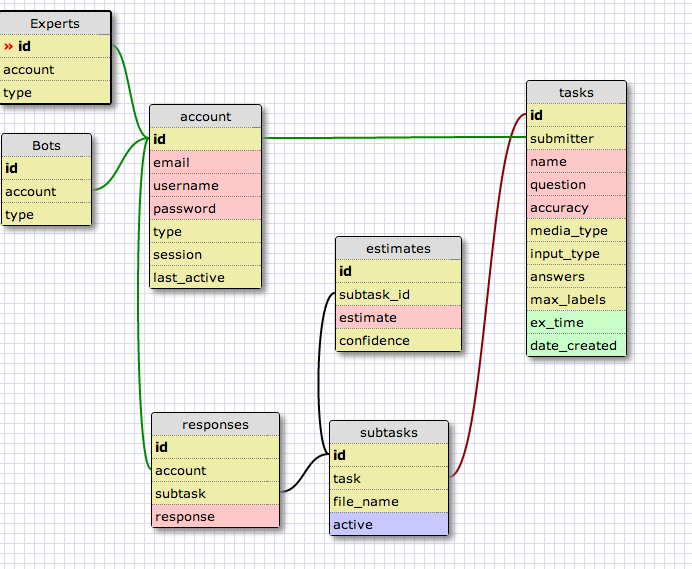
\includegraphics[width=\linewidth]{images/schema.png}
\caption{Database Schema}
\label{default}
\end{center}
\end{figure}

When adding tasks, if the database transaction succeeds, a folder is made in our group
directory of the form TaskFiles/[taskID]/ . Upon adding subtasks to this task, the
file contents are outputted to the taskID folder. We support Zip uploading via
Java's java.util.zip package which lets us output multiple file entries easily.
The URL to write to is specified by an absolute path to our project dir. Of course, this would
have to be modified if we were to deploy our application to an environment outside DoC.

Upon receiving a response from the client for a subtask, its value is passed into our
EM Algorithm and the annotator's information is updated, along with the answer for the
subtask as described later.

Tomcat allows us to specify running the servlet container over SSL. This means
that any information passed between client and server is unable to be intercepted
by an intruder. This is implemented through parameters in our server.xml specifying
the port for which SSL connections should be sent (55550 at present). We also have
an http connection at port 8080 for users who don't wish to use SSL, however this port can
easily be blocked if the decision is made to require users to authenticate via SSL.

\subsection{Algorithm}

\subsection{Data Processing}

Once clients have submitted their tasks and the crowd are submitting answers, our goals are:
\begin{enumerate}
\item To estimate the correct annotation for each subtask based on crowd annotations and their respective likelihoods of being correct.
\item To use crowd annotations to better our understanding of the accuracy of a crowd
\end{enumerate}

These goals can be achieved with the `Expectation-Maximisation algorithm'. We have adopted this algorithm for the processing of annotations, generalised it to work over a variety of task types and implemented it to function efficiently in an online environment.\\

\subsubsection{EM-Algorithm overview}

The a EM algorithm models the system as a hypothesis, h, and new evidence, Y, which is a set independent instances with observed data, X, and unobserved data, Z.

For our particular case we have a set of subtasks, S, with correct annotations, $Z_{s}$; a set of annotators, J, with accuracies $A_{j}$ and labels $L_{ij}$ from these annotators to subtasks

It then iterates through two steps to revise this hypothesis so that it converges on the most likely hypothesis for the state of the system.\\

Expectation Step:\\
You calculate P(Z) values using the X assuming the current hypothesis holds. In our case Z are the correct annotations for each subtask, X are the provided labels and the current hypothesis is the annotator`s accuracy. [1]\\

$ p(z_{i}) = p(z_{i}|\zeta) \prod p (l_{ij} | z_{i} a_{j}) $ (1)\\

where $p(z|\zeta)$ is our prior belief of $p(z)$.\\

Maximisation Step:\\
You replace the current hypothesis h with the most likely hypothesis assuming that the Z = E[Z]. This will mean that we have to calculate our most likely accuracies for the system based on the expected correct annotations calculated from the previous step.\\

$ Q(a_{j},a\prime_{j}) = \log p(a_{j}|\alpha_{j}) + \sum E_{z_{i}} [\log p (l_{ij} | z_{i} a_{j})]$ (2)\\

\subsubsection{Annotation types}

Our framework deals with a variety of subtasks that have different annotation types and models for accurate behaviour.

We model each of the subtasks with a different conjugate prior and model for accurate behaviour.\\

%\renewcommand{\arraystretch}{1.5}
\begin{table}[htdp]
\caption{Subtask models [2]}
\begin{center}
\begin{tabular}{|p{2cm}|p{5cm}|p{4cm}|p{4cm}|}
Subtask type & Description & conjugate prior & likelihood \\
\hline
Binary & An annotator can respond either true or false & $Beta(\alpha_{j}^{0}, \beta_{j}^{0})Beta(\alpha_{j}^{1},\beta_{j}^{1})$, where $\alpha_{j}^{0/1}$ are the negative and positive successes and $\beta_{j}^{0/1}$ are the failures.& $p(l_{ij} = z_{i} = 1 | a_{j}) = a_{j}^{1}$ $p(l_{ij} = z_{i} = 0 | a_{j}) = a_{j}^{0}$\\ [2cm]

Multivalued & An annotator must categorise the subject into one of a range of categories D & $Beta(\alpha, \beta)$, where $\alpha$ is the number of successes and $\beta$ the failures.  &  $p(l_{ij} = z_{i}| a_{j}) = a_{j}$ $p(l_{ij} \ne z_{i} | a_{j}) = \frac{1 - a_{j}}{D - 1}$\\ [1cm]

Continuous & An annotator must respond using a tuple from an N-dimensional number line & as above &  $p(l_{ij} | z_{i} a_{j}) = a_{j} p(l_{ij}|honest) + (1- a_{j}) p(l_{ij}|random)$, where the probability of an honest label is given by $\mathcal{N}(l_{ij}, \sum)$ for a given variance and the random probability is uniform over the response space.\\
\end{tabular}
\end{center}
\label{models}
\end{table}

\subsubsection{Online Considerations}

The online implementation of this algorithm is different in that it does not compute the expected labels as a batch job but instead has to observe several instances, one at a time, over a long period of time.

It also exploits discrimination. Expert annotators are asked first to respond to subtasks in order to reduce the total number of labels required. Since experts are likely to be the minority this technique is important since it makes sure that their annotations are taken into account [3].

We carry this out by checking the variance of our estimate for the most likely accuracy of an annotator. A large variance would suggest that we do not yet have enough information to judge an annotator. When the variance is small enough, we will test the accuracy against the criteria below.\\

\begin{table}[htdp]
\caption{default}
\begin{center}
\begin{tabular}{|c|c|}
Subtask type & criteria\\ \hline
Binary & \shortstack{$\frac{\Phi^{-1}(a_{j}^{0}) - \Phi^{-1}(1 - a_{j}^{1})}{2} > 2$ \\ i.e an annotator's sensitivity index [1] is greater than 2}\\
Multivalued & $a_{j} > 0.85$\\ 
Continuous & $a_{j} > 0.85$\\
\end{tabular}
\end{center}
\label{default}
\end{table}%

\subsubsection{Implementation details}

\begin{figure}[htbp]
\begin{center}
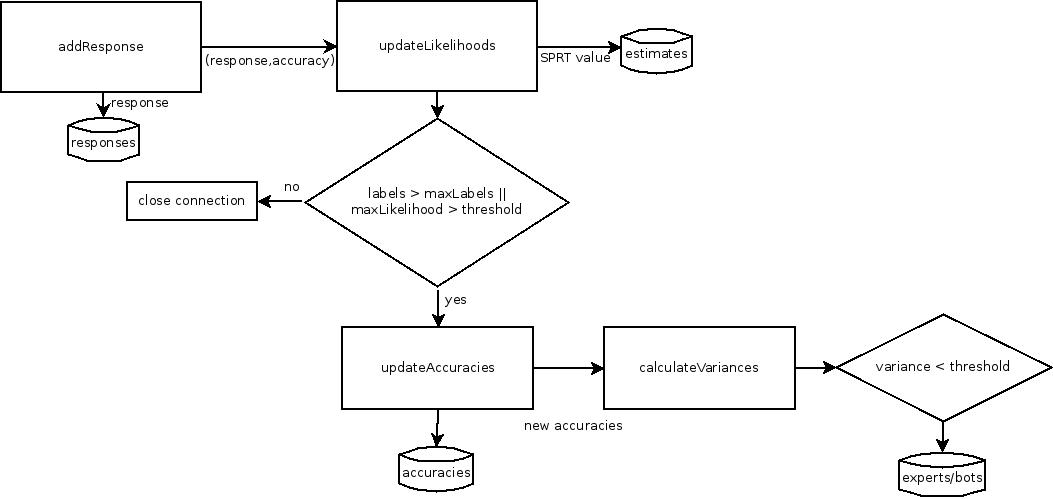
\includegraphics[width=\linewidth]{flow.jpg}
\caption{algorithm}
\label{default}
\end{center}
\end{figure}


E step\\

To calculate (1), values for the Sequential Probability Ratio Test [4] for each hidden value Z are stored in the database. Since the value is the sum of a sequence, the stored value can simply be increased by the new value. At this point each value is tested with the threshold to see if the maximum likelihood is great enough. At this point the M step will begin.\\

M step\\

To compute the new accuracy (2), the prior accuracy needs to be modelled as a distribution stated in figure 1 and the expected accuracy is calculated assuming the correct label is the most likely one from the last step.

The new accuracy would be the peak of the equation (2). To avoid using numerical methods to estimate the peak we write the Bayes estimate as a convex combination of the prior and the data [5]. This way we get a formula for the expected accuracy that can be computed in constant time:\\

\begin{table}[htdp]
\caption{Bayes estimate}
\begin{center}
\begin{tabular}{|c|c|c|}
Subtask type & Convex combination & $\theta_{mle}$\\ \hline

Binary & $ E(a_{j}^{k}) = \gamma \frac{\alpha_{j}^{k}}{\alpha_{j}^{k} + \beta_{j}^{k}} +  (1 - \gamma)\theta_{mle}$, only for affected k & 1 if $l_{ij} = z_{i}$, 0 otherwise\\

Multivalued & $ E(a_{j}) = \gamma \frac{\alpha_{j}}{\alpha_{j} + \beta_{j}} +  (1 - \gamma)\theta_{mle}$ &1 if $l_{ij} = z_{i}$, 0 otherwise\\

Continuous & $ E(a_{j}) = \gamma \frac{\alpha_{j}}{\alpha_{j} + \beta_{j}} +  (1 - \gamma)\theta_{mle}$ & \shortstack{$\frac{\mathcal{N}(l_{ij}| z_{i}, \sum)}{\mathcal{N}(l_{ij}| z_{i}, \sum) + \lambda^{-1}}$ \\ where $\lambda$ is the response space}\\
\end{tabular}
\end{center}
\label{def}
\end{table}%

where $\gamma = \frac{\alpha_{j}^{k} + \beta_{j}^{k}}{\alpha_{j}^{k} + \beta_{j}^{k} + 1}$ 

Once the accuracies have been updated we must check the variance of the posterior accuracy. In the cases where the accuracy is modelled as a single beta distribution, multi valued and continuous, is trivial:

In the binary case the accuracy is modelled as a product of two dependant distributions therefore the variance must be estimated. We fit the peak to a multivariate Gaussian curve to estimate the posterior`s variance.

If we are confident in our knowledge of the annotator we test its accuracy against the criteria and store any new data about experts and bots in the database.\\

%[1] – Machine Learning Tom M Mitchell
%[2] - A Compendium of Conjugate Priors - John D. Cook
%[3] – Online crowdsourcing: rating annotators and obtaining cost-effective labels - Welinder Perona
%[4] - Sequential tests of statistical hypotheses – Wald
%[5] – Bayesian inference for simple problems - Simon Jackman
 
 
%%%%%%%%%%%%%%%%%%%%%%%%%%%%%%%%%%%%%%%%%%%%%%%%%%%%%%%%%%%%%%%%%%%%%%%%%%%%%%%% 
\section{Software Engineering}
\subsection{Technologies}
\subsubsection{Languages}
We used the following languages during the development of Crowdtrust:
\begin{itemize}
\item
\emph{Java} - All of our group has a lot of experience with Java, which gave it a huge appeal to us.
On a project with as large a scope as ours, we decided it was important to be able
to understand the logic of our code without being confused about the syntax or
constraints of the language.

It also gave us the comfort of (partial) type safety in our large project. This meant that changes could be made more confidently and tools could easily `understand' our code.

Java also has an in built servlet class which we
decided would be ideal for the client-server interactions 
\item
\emph{PSQL} - This was chosen for out database language because we have all been
taking a databases course this term which has involved writing many PSQL queries,
this makes it the obvious choice as everyone was familiar and comfortable with 
\item
\emph{HTML} -
HTML is the standard web markup language. HTML5 initially came out in 2011 with many
browsers now supporting a large majority of its features. As a result of the wide
adoption of HTML5 amongst browsers, and the feature improvements over HTML4/XHTML1.1
we decided upon HTML5 being the ideal language.
\item
\emph{JSP} -As stated above, Java was our ideal programming language to develop in. As Java
has servlet support built in, we used servlets on our server side. As we developed
the website more, we found jsp to be the ideal language to connect with our database
and communicate with our server.
\item
\emph{CSS3} - We utilised CSS3 to provide the layout information to our website. It is one of the
most commonly used styling methods for HTML5 pages
\end{itemize}
\subsubsection{Development Tools}
We used the following tools during the development of Crowdtrust:
\begin{itemize}
\item
\emph{Eclipse} - 
Eclipse is the standard development tool we use for Java. Our build tool also
had built in plugins to support making eclipse projects.
\item
\emph{Maven} -As a result of our decision to use Java, we utilised Apache Maven as
our build tool. Initially we were using Make to build our project as our entire team had 
previous experience with it, however almost immediately we ran into problems with
class dependencies and other project imports. One of our team had previously utilised
this tool successfully for a Java project and was proficient enough with it to apply
it to our project. The use of Maven allowed us to easily work on separate parts of
the project, combining our code via git, and then importing the project into eclipse
for easy coding.

Maven also provides in built support for web applications. With the Maven archetype:generate
goal, we were able to generate a project structure which was both recognisable by
Maven, enabling the build process, and able to generate a valid war file to run our webapp
from. Using the Maven Tomcat7 plugin, it was possible to swiftly compile, test, package and
then deploy our project to a tomcat server, providing instant feedback on changes we made. 

\item
\emph{Microsoft Expression Web 4} - 
To develop our website, we initially set out to use Microsoft Expression Web 4.
Initially it seemed useful as our website consisted of mainly html pages and so
could use the IDE to assist in coding. We moved away from using the tool, however, and began coding by hand. This was because we migrated to jsp. The in built support for jsp was non existent, and many of the `features' of the tool became a hindrance.
\end{itemize}
\subsubsection{Libraries}
We used the following libraries in our project:

\begin{table}[htdp]
\caption{Libraries Used}
\begin{center}
\begin{tabular}{|p{4cm}|p{3cm}|p{3cm}|p{6cm}|}
Location & Name & Version & Use \\
\hline
junit                                   & junit               & 4.8.1               & Used for creating Junit tests \\
org.glassfish.main.\\jdbc.jdbc-ra.jdbc40  & jdbc40            & 4.0-b33             & Used to connect Java with PSQL \\
org.ancoron.postgresql                  & org.postgresql      & 9.1.901.jdbc4.1-rc8 & Used to provide database functionality \\
commons-fileupload                      & commons-fileupload  & 1.2.2               & Used to upload files to the database \\
javax.servlet                           & javax.servlet-api   & 3.0.1               & Used to create Tomcat servlets \\
org.apache.commons                      & commons-math3       & 3.0                 & Used model the distributions in the algorithm \\
be.ac.ulg.montefiore.run                & jahmm               & 0.6.2               & Used to model distributions not contained in the apache library, i.e. MultiGaussianDistribution \\
opensymphony                            & sitemesh            & 2.4.2               & Used to create web templates \\ 
org.apache.commons                      & commons-lang3       & 3.1                 & Used for string processing 

\end{tabular}
\end{center}
\label{libs}
\end{table}

\subsection{Project Management}
\subsubsection{Design Practices}
We adopted several techniques taught to us in the Software Engineering Course
given by Dr. Robert Chatley.
The practices we adopted:
\begin{itemize}
\item 
\emph{Pair Programming} - As a group we have always been strong advocates of pair
		 programming. We adopted a system where pairs alternate to test each other`s code. 			 Criticising each other is an essential part of pair programming
		 having to justify your choices makes you think about them more, it also 
		 stops you going off track and getting too invested in an idea. Having
		 one partner thing about ideas and structure and one partner code also speeds
		 up development.
		 
\item 
\emph{Sitting and coding together} - Although all of us had different timetables,
			we tried to sit down and code together as often as possible, so all
			of us knew what was going on and no one was out of the loop. Also, while
			working together, we could easily have discussions about problems we
			were facing.
\item 
\emph{Having an informative workspace} - As 4 of us live together and the other
			person lives very close by, we would usually meet up to code in a 
			dedicated room, complete with a whiteboard and a spare wall for post-it
			notes. Being together in such a close environment made it easy to bounce
			ideas off of each other or ask advice, sometimes you don't even need advice
			you simply need to speak out loud about your problem.

\item 
\emph{Stand up meetings} - Every time we coded together we would spend ten minutes
			stood around the whiteboard talking about where everyone was up to and what needed to
			be done that day. These meetings were invaluable it helped to keep everyone on track and
			focussed, it was far easier to see why what you were doing needed to be done, who needed it done 
			and how it was going to fit into the project as a whole.

\item
\emph{Whiteboard} - We own a large whiteboard which became one of our most treasured tools. Diagrams and plans 
					need to be seen and easy consult, having them tucked away on some professional software
					just means they're easy to forget about and hard to alter. We would get together and do
					system designs on the whiteboard they would stay on there for a while (whilst they were in a state of
					flux and regularly altered) and then once we were sure they would be committed to paper and stuck on the wall.
					The whiteboard was also used to hold workflow lanes which held the jobs to be done and how complete they were, 
					different pens were used to indicate different things about the job. Once a job was complete the person who
					completed it would go up to the board and sign it off, as well as committing it on git.
					
\begin{figure}[H]
\begin{center}
\includegraphics[width=\linewidth]{images/whiteboard.jpg}
\caption{Team whiteboard during a brain storming session}
\label{default}
\end{center}
\end{figure}  		
			
\end{itemize}

\subsubsection{Collaboration Tools}

In order to complete the project, we have made use of several tools which have
allowed us to collaborate our work efficiently. These are discussed below.

\begin{itemize}
\item 
\emph{Git} - Git was used as our version control system. All of us had previously
used git, so we were comfortable using it. Besides familiarity, there were
many other points which encouraged us to use git instead of other version control
systems. Firstly, since we would be working in several different places, such as
at home and in labs, we wanted a decentralised repository, which was provided
by using git. Git also allowed us to branch from the master branch when we were
working on something new, which was very convenient. Code from branches was
merged with the master branch only after thorough testing of the code.
\item 
\emph{Github} - We used Github to track the progress of our project over the course
of the project development. Being able to read our detailed commit messages
allowed us to know where everyone was at with their part of the project. Again,
as with git, Github was available to us anywhere, so that was an added advantage
for using it.

We exploited branches to develop features without disruption and committed regularly
to avoid large conflicting commits.
\item 
\emph{Google+} - To complete our report over the Christmas break, communication was going
to be a problem as all of us were in different places. To tackle this problem,
we decided to have regular meetings on Google Plus. We would have them every 2
days, where we would discuss what we had accomplished, and what we would be working
on next. At the end, it worked out really well.
\item 
\emph{Skype, IM} - At points, people would be working in pairs and such, so using
these means of communication were useful as we could not be present with one
another at all times.
\item
\emph{Database Token} - There were times during the development where testing the
framework and algorithm conflicted with each other as regards the database. The solution 
was a database token (which took the form of a can of vanish carpet cleaner) when someone
wanted to have the database in isolation he would ask for the token when would be physically
passed to him, during that time no one was allowed to write to the database.

\end{itemize}


\subsubsection{Teamwork and Work Division}
Before beginning coding, the group sat down and discussed the major chunks
which had to be completed. We then evaluated where each of our strengths
and weaknesses lied, and then everyone took responsibility of a part of the
project. We also decided that wherever possible, we would try to work with 
someone else. Although everyone had taken charge of a specific part of the
project, they were not bound to that part, as they could contribute towards
other people's parts as well.

Below we describe what people were mainly in charge of:


\begin{table}[H]
\caption{Jobs Assigned}
\begin{center}
\begin{tabular}{|p{2cm}|p{5cm}|p{7cm}|}
Name & Job & Justification\\
\hline

Giovanni Charles & Algorithm development and testing                                       &
Giovanni felt he had a strong ground in mathematics and states which suited him to the role
\\ 
John Walker      & Algorithm testing and development                                       &
John has worked closed with Giovanni in the past and they have proven themselves as a productive team.
John also had experience with testing from his summer internship. 
\\
Adam Fiksen      & Website development and client-server interaction, Maven configuration  &
Adam had experience with Maven from his summer internship and offered to set up Maven. Adam
felt from his distributed systems course he had a good knowledge of client server interaction.
\\
Sahil Jain       & Database interaction and structure                                      &
Sahil had a lot of experience with PSQL and databases during his summer internship which he felt
suited him to the roll.
\\
Ryan Jackson     & Handling crowd questions and responses                                  &
Ryan is good at seeing the bigger picture and producing well generalised code, as this was a large
unfamiliar part of the project he felt comfortable in the position.
\\

\end{tabular}
\end{center}
\label{jobs}
\end{table}

%%%%%%%%%%%%%%%%%%%%%%%%%%%%%%%%%%%%%%%%%%%%%%%%%%%%%%%%%%%%%%%%%%%%%%%%%%%%%%%%
\section{Evaluation}
%summarise testing procedures (+ relevant testing results)
\subsection{Testing}
\subsubsection{Algorithm}
Testing the algorithm required creating Java classes to model an annotators behaviour, an annotator $j$ was given three behaviours:

\begin{enumerate}
\item
[3]
\emph{Binary behaviour} - This modelled how well a user could answer yes/no questions such as 'Is the bird in this image $i$ a robin?'. The target
value $z_{i}$ and label produced $l_{ij}$ can take on values $z_{i}, l_{ij} \in \{0, 1\}$ An annotators ability to answer questions was 
parameterised by a true positive rate $a_{j}^{1}$ and a true negative rate $a_{j}^{0}$.

Binary answers are modelled in a 
signal threshold manner, When an annotator is presented with a question he generates a signal in his brain $x_{i}$ if this signal is above
a threshold $t_{j}$ then the annotator returns a positive 'yes' answer, otherwise they return a negative 'no' answer. The threshold represents
how bias the annotator is toward a particular answer, a threshold approaching 1 represents a predisposition towards a yes answer and 0 a 
negative answer.
%Talk about where we got threshold from

When the annotator was given a question
we would look at some testing information which we attached to the question to find out what the actual answer $z_{i}$ was, we would then generate
the appropriate Normal distribution to represent his signal:

$p(x_{i} | z_{i} = k) \sim \mathcal{N}(\mu_{j}^{k} , 1)$

A random sample was taken from the appropriate normal distribution compared to the threshold and the annotators answer was returned. 
[3]
\item
\emph{MultiValued Behaviour} - This modelled how well the annotator could respond to categoric questions such as 'How many birds are in this picture?' 

Following the advice laid out in the paper we looked into creating a confusion matrix to model how often an annotator confuses one particular answer with another, however we decided this wouldn't really be appropriate as one confusion matrix for all multi valued questions would be misleading for questions with a varying number of options. 

In the end we chose to follow the method they used in the paper which was to assign the annotator a 'correctness' rate this represented how often he got a question right. We would then generate a uniformly distributed random variable to determine wether they answered the question correctly and return their answer.

[3]
\item
\emph{Continuous Behaviour} - We chose to model bounding boxes for our continuous question. A bounding box is a tight fitting box surrounding
a portion of an image represented by its top left $(x_{1}, y_{1})$ and bottom right $(x_{2}, y_{2})$ co-ordinates. 

%Fill in the rest of this

\end{enumerate}

A number of taks and subtasks were then generated and entered into the database along with a number of annotators. Subtaks were selected at random
and given to annotators and their answers were stored in the database. A comparrison was then drawn between the ability of the annotators and
their estimated ability according to the algorithm. Below are some results of our testing explained in the figures. 


\begin{figure}[H]
\begin{center}
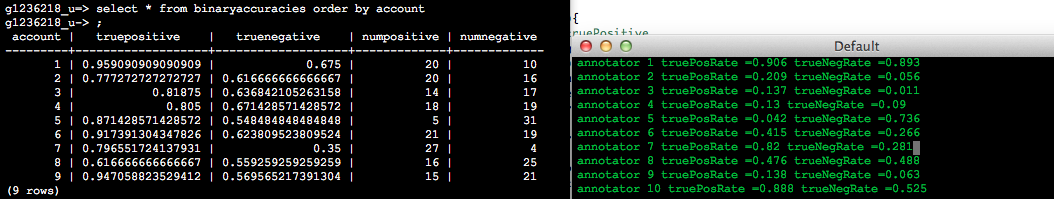
\includegraphics[width=\linewidth]{images/test1.png}
\caption{comparisons of estimated binary accuracies with true binary accuracies. This was done over 10 synthetic accuracies over 10 synthetic subtasks}
\label{default}
\end{center}
\end{figure}


\begin{figure}[H]
\begin{center}
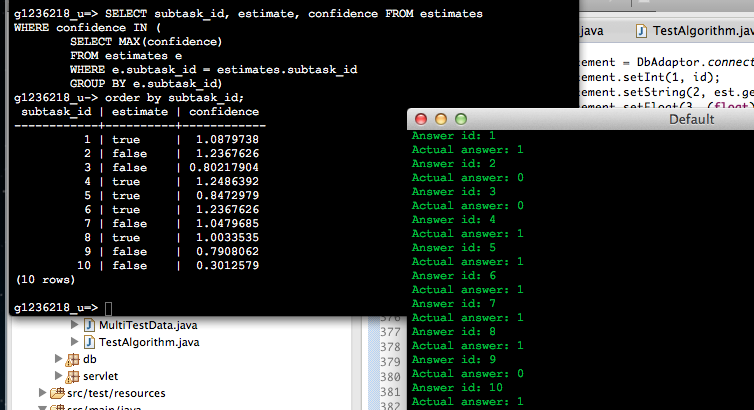
\includegraphics[width=\linewidth]{images/test2.png}
\caption{comparisons of estimated true binary values with true binary values. This was done over 10 synthetic accuracies over 10 synthetic subtasks}
\label{default}
\end{center}
\end{figure}

The following JUnit tests from the corresponding test packages were run on every build:

\subsubsection{Validity}
Validity testing ensures our system can handle erroneous events.
\begin{itemize}
\item testAddNullSubTask
\item testAccuracyIsBetweenZeroAndOne
\end{itemize}
\subsubsection{Security}
Security testing ensures our system conforms to the appropriate security standards, below are the security tests we carried out:
\begin{itemize}
\item testUserRequestUnAuthTaskId
\item testUserSendUnAuthResponse
\end{itemize}
\subsubsection{Scaleability}
Scalability testing ensures the system can handle increased demand, below and the scalability tests we carried out:
\begin{itemize}
\item testAlgorithm (annotators > 10000)
\item testAlgorithm (tasks > 10000)
\end{itemize}
\subsubsection{Performance}
Performance testing ensures the system performs in a timely manner, below are the performance tests we carried out: 
\begin{itemize}
\item batchUploadAccuracies (time < 500msec)
\item concurrentResponses (threaded calls of addResponse)
\end{itemize}
\subsubsection{Correctness}
Correctness testing ensures the system outputs what it is supposed to, below are the correctness tests we carried out:
\begin{itemize}
\item testExperts (expert lists are correct)
\item testGetRandomSubtask (all generated subtasks are unanswered and match the id)
\end{itemize}
\subsubsection{End To End - algorithm package}
End to end testing ensures a process makes its journey correctly through the system, below are the end to end tests we carried out:
\begin{itemize}
\item testAlgorithm
\end{itemize}

%Evaluate your deliverables in terms of performance usability
%usefulness, (how successful was the project?)

%%%%%%%%%%%%%%%%%%%%%%%%%%%%%%%%%%%%%%%%%%%%%%%%%%%%%%%%%%%%%%%%%%%%%%%%%%%%%%%%
%\newpage
\section{Conclusion and Future Extensions}
%Say what you've concluded from doing the work and how you'd build on it

%%%%%%%%%%%
\subsection{Conclusion}
%%%%%%%%%%%
\subsubsection{Achievements}
The algorithm was a success in that it generalised the EM algorithm proposed in 

%%%%%%%%%%%
\subsection{Future Extensions}

%%%%%%%%%%%%%%
\subsubsection{Tagging}
Tagging could be used to improve the efficiency of our algorithm, for instance when a user signs up to the website he could provide a list of his interests such as football or birdwatching and when a client submits a task to the website he uses a similar tagging system to record what his task is related to. If a user provides an answer to a task which is in line with his interests then it is more likely his answer will be correct the algorithm would take this into account when calculating how sure it is of an answer. This will result in less people having to be asked for each question which will improve turnaround time for jobs submitted to the system. 


%%%%%%%%%%%%%%
\subsubsection{Dynamic Pricing Model}
If you do any reading into Amazons Mechanical Turk it's not long before you will meet some criticisms on the way they pay their workers with some
even likening it to an electronic sweat shop. The average wage for a worker is around \$2 far below the minimum wage and the average payment for 
a task is around 30 cents, whats more the requestor is under no obligation to pay the worker unless he is completely satisfied this is often abused
with companies simply choosing not to pay the workers. Workers really have no control over their wage and the amount they are paid simply 
reflects how quickly they can complete tasks, crowdtrust could be used to change this.

With crowdtrust you keep track of an annotators 'expertise' and so you can return an answer to a task with a measure of how sure you are of its
correctness, this means users will not have to submit tasks multiple times to validate them this saves the user money and as a result some of this
saving could be passed on to the annotators to reward them for being experts.   

%%%%%%%%%%%%%%
\subsubsection{Mobile Access}
Although Mechanical Turk has over 500000 workers registered 80\% of HITs are performed by around 20\% of the workforce and this isn't a 
particularly large number. The reason for this we believe is the pay, if you're at home there are many things you'd rather be doing than sitting
if front of your computer for \$2 an hour. However if you're stuck on a 4 hour train journey from Newcastle back to London for university and
you could have access to a crowdtrust app on your phone you may be far more willing to sit there and earn \$8. We believe a mobile app would 
greatly increase the user base and therefore the turn around time for tasks submitted to the system. 

%%%%%%%%%%%
\subsection{Hybrid Crowdsourcing}
This was offered as a separate project by our supervisor, hybrid turk seeks to use both computer and human processing to complete a task. A computer starts a processing task and when it reaches something that needs a human touch for example, `For example, for navigation through image recognition users may be asked to take pictures which are then processed automatically. But due to the difficulty of the task in cases where image analysis algorithms do not give sufficiently accurate results, other users may be asked to label the content of the image (or parts of the image), which can then be further processed automatically'.

Implementing this would involve modelling a prior probability distribution for $p(z|\zeta)$ and have it taken as an input from a client. At the moment this is modelled as a uniform distribution.[11]
% from emils project specification

%%%%%%%%%%%%%%%%%%%%%%%%%%%%%%%%%%%%%%%%%%%%%%%%%%%%%%%%%%%%%%%%%%%%%%%%%%%%%%%%
\section{Appendix}

%%%%%%%%%%%%%%%%%%%%%%%%%%%%%%%%%%%%%%%%%%%%%%%%%%%%%%%%%%%%%%%%%%%%%%%%%%%%%%%%
%\newpage
\begin{thebibliography}{99}

\bibitem{one}
  Tom M Mitchell,
  \emph{Machine Learning}.
  Mcgraw-Hill International,
  New Edition,
  1997.
  
\bibitem{two}
  John D. Cook,
  \emph{A Compendium of Conjugate Priors}.

\bibitem{three}
  Welinder Perona,
  \emph{Online crowdsourcing: rating annotators and obtaining cost-effective labels}.
  
\bibitem{four}
  Wald,
  \emph{Sequential tests of statistical hypotheses}.
  
\bibitem{five}
  Simon Jackman,
  \emph{Bayesian inference for simple problems}.
  
\bibitem{six} 
  Michael Neilson,
  \emph{TedXWaterloo Open science}.
  http://www.youtube.com/watch?v=DnWocYKqvhw.

\bibitem{seven}
	Elinor Mills,
	\emph{CNN news}.
	http://news.cnet.com/8301-10784\_3-9782813-7.html.   
	
\bibitem{eight}
	\emph{Mechanical Turk}.
	https://www.mturk.com/mturk/welcome.	
	
	
\bibitem{nine}
	\emph{ProPublicas guide to Mechanical Turk}.
	http://www.propublica.org/article/propublicas-guide-to-mechanical-turk.
	
\bibitem{ten}
	\emph{MicroWorkers}.
	http://microworkers.com/faq.php.
	
  \bibitem{eleven}
	\emph{Dr Emil Lupu}.
	http://doc.ic.ac.uk.
  
  %[1] – Machine Learning Tom M Mitchell
%[2] - A Compendium of Conjugate Priors - John D. Cook
%[3] – Online crowdsourcing: rating annotators and obtaining cost-effective labels - Welinder Perona
%[4] - Sequential tests of statistical hypotheses – Wald
%[5] – Bayesian inference for simple problems - Simon Jackman

\end{thebibliography}

\end{document}

